% -*- coding: utf-8 -*-
\documentclass{beamer}
\usepackage[utf8]{inputenc}

\usetheme{complang}

% Have Page n/N in the lower left corner
% \setbeamertemplate{footline}
% {%
% \begin{beamercolorbox}[wd=0.5\textwidth,ht=3ex,dp=1.5ex,
%    leftskip=.5em,rightskip=.5em]{author in head/foot}%
% \usebeamerfont{author in head/foot}%
% \insertframenumber/\inserttotalframenumber\hfill\insertshortauthor%
% \end{beamercolorbox}%
% \vspace*{-4.5ex}\hspace*{0.5\textwidth}%
% \begin{beamercolorbox}[wd=0.5\textwidth,ht=3ex,dp=1.5ex,
%    left,leftskip=.5em]{title in head/foot}%
% \usebeamerfont{title in head/foot}%
% \insertshorttitle%
% \end{beamercolorbox}%
% }

%\usepackage{pifont}
%\usepackage{amstext}
%\usepackage{amsmath}
%\usepackage{logic}
% \usepackage{proof}
\usepackage{xcolor}
\usepackage{listings}
\usepackage{hyperref}

\usepackage{tikz}
\usetikzlibrary{arrows,automata,positioning}
\usetikzlibrary{fit}
\usepackage{drawproof}

% Colors
\definecolor{myblue}{rgb}{0.089, 0.089, 0.58}
\definecolor{myred}{rgb}{0.77, 0.05, 0.16}
\definecolor{mygreen}{rgb}{0.05, 0.77, 0.16}
\definecolor{myyellow}{rgb}{0.77, 0.77, 0.16}

\setbeamercolor{local structure}{fg=black}

% Arrows
\newcommand{\redarrow}{{\color{myred} \Pisymbol{pzd}{217}}}
\newcommand{\redresarrow}{{\large\color{myred} \Pisymbol{pzd}{229}}}
\newcommand{\ra}{\hspace{1cm}\redarrow}
\newcommand{\rad}{\begin{rotate}{-90}{\Large\color{myred} 
      \Pisymbol{pzd}{225}}\end{rotate}}
\newcommand{\fatredarrow}{\hspace{1cm}{\color{myred}\Large \Pisymbol{pzd}{225}}}

%% Result
%\newcommand{\resbox}[1]{
  %\begin{itemize}
  %\item[\redresarrow] #1
  %\end{itemize}
%}


%-------TITLE-----------------------------------------------------------
\title{
  Space and Congruence Compression of Proofs  
}

\author{
  Andreas Fellner
}

\institute[TU Wien]{
	
\includegraphics[width=3cm]{figures/INF_Logo_typo_grau.png} \hspace{1cm} 
	
\includegraphics[width=2cm]{logo-complang} \\[1cm]
	\Large{European Master in Computational Logic} \\[1cm]
  %\Large{Computational Logic}
  %\begin{tabular}{cc}
    %
\includegraphics[width=3cm]{figures/INF_Logo_typo_grau.png} &
		%\begin{tabular}{c}   
      %European Master in \\
      %Computational Logic \\
      %\\
      %\\
    %\end{tabular} \\
		%
\includegraphics[width=2cm]{logo-complang} & \\   
  %\end{tabular}
}

\date{Master Thesis Presentation\\ Vienna, $23^{rd}$ of September 2014}
%-----------------------------------------------------------------------

\begin{document}
\rm % Use ROMAN fonts

%\section{}

\begin{frame}

\maketitle

\end{frame}

%\section{Congruence}

\begin{frame}

\frametitle{Example}

\begin{block}{Knowledge}
	\begin{enumerate}
		\item $f(a) = a$
		\item $a = b$
		\item $b = f(b)$
		\item $f(a) \neq f(b)$
	\end{enumerate}
\end{block}

%\begin{itemize}
%\uncover<2->{\item Unsatisfiable!\\}
%\uncover<3->{\item Proof: Equality is transitive, therefore from $f(a) = a$, $a = b$ and $b = f(b)$ follows $f(a) = f(b)$, which contradicts $f(a) \neq f(b)$}
%\uncover<4->{\item Another Proof: $f(.)$ is a function, therefore from $a = b$ follows $f(a) = f(b)$, which contradicts $f(a) \neq f(b)$}
%\end{itemize}

\uncover<2->{{\color{red} Unsatisfiable!\\}}
\uncover<3->{
	\begin{block}{Proof} 
		Equality is transitive, therefore from $f(a) = a$, $a = b$ and $b = f(b)$ follows $f(a) = f(b)$, 
		which contradicts $f(a) \neq f(b)$
	\end{block}
}
\uncover<4->{
	\begin{block}{A different Proof} 
		$f(.)$ is a function, therefore from $a = b$ follows $f(a) = f(b)$, 
		which contradicts $f(a) \neq f(b)$
	\end{block}
}
\end{frame}

\begin{frame}

\frametitle{Definitions}

\uncover<2->{
\begin{block}{Ground Terms}
	\begin{itemize}
		\item Constants $a,b,c, \ldots$
		\item Compound Terms $f(t_1,\ldots,t_n)$
	\end{itemize}
\end{block}
}
\uncover<3->{
\begin{block}{Congruence Relation}
	\begin{itemize}
		\item \makebox[2cm]{Reflexive:\hfill} $t = t$
		\item \makebox[2cm]{Symmetric:\hfill} $s = t \Rightarrow t = s$
		\item \makebox[2cm]{Transitive:\hfill} $t_1 = t_2 \ldots t_{m-1} = t_m \Rightarrow t_1 = t_m$
		\item \makebox[2cm]{Compatible:\hfill} $\forall_i: t_i = s_i \Rightarrow f(t_1,\ldots,t_n) = f(s_1,\ldots,s_n)$
	\end{itemize}
\end{block}
}
\uncover<4->{
\begin{block}{Congruence Closure $R^*$ of $R$}
	\begin{itemize}
		\item Smallest Congruence Relation containing $R$
	\end{itemize}
\end{block}
}
\uncover<5->{
\begin{block}{Explanation for $s = t$}
	\begin{itemize}
		\item Set of equations $E$, such that $(s,t) \in E^*$
	\end{itemize}
\end{block}
}
\end{frame}

\begin{frame}

\frametitle{Example continued}

\begin{block}{Knowledge}
	\begin{enumerate}
		\item $f(a) = a$
		\item $a = b$
		\item $b = f(b)$
		\item $f(a) \neq f(b)$
	\end{enumerate}
\end{block}

\uncover<2->{
\begin{block}{Explanation for $f(a) = f(b)$}
	$\{$ \visible<2>{$f(a) = a,$} \uncover<2->{$a = b$} \visible<2-3>{$,b = f(b)$} $\}$
\end{block}
}
\uncover<5->{Short explanation $\leadsto$ short proof}
\end{frame}

\begin{frame}

\frametitle{Short Explanation Decision Problem}

\centering Given a set of input equations $E$, a target equation $s = t$ and $k \in \mathbb{N}$, does there exist an explanation $E' \subseteq E$ of $s = t$ with $|E'| \leq k$?
%\centering Given a set of input equations $E$, a target equation $s = t$ and $k \in \mathbb{N}$, does there exist a set $E' \subseteq E$ with $|E'| \leq k$ and $E'$ is an explanation for $s=t$?

\uncover<2->{\vspace{1cm} \centering\alert{\textbf{NP-complete}}}

\end{frame}

\begin{frame}

\frametitle{NP-completeness proof sketch}

\begin{block}{From a propositional logic formula $\Phi$ obtain $\ldots$}

	\begin{itemize}
		\item a set of equations $E_{\Phi}$
		\item a target equation $s_{\Phi} = t_{\Phi}$
		\item $k_{\Phi} \in \mathbb{N}$
	\end{itemize}
\end{block}

\begin{block}{such that $\ldots$}
	$\Phi$ is satisfiable if and only if there is an explanation $E' \subseteq E_{\Phi}$ of $s_{\Phi} = t_{\Phi}$ with $|E'| \leq k_{\Phi}$
\end{block}

%\begin{itemize}
	%\item Translate propositional logic formula $\Phi$
%\end{itemize}

\end{frame}

\begin{frame}

\frametitle{NP-completeness proof sketch example}

\begin{block}{Formula}
$$(x_1 \vee x_2 \vee \neg x_3) \wedge (\neg x_2 \vee x_3) \wedge (\neg x_1 \vee \neg x_2)$$
\end{block}
\only<1-8>{
\begin{block}{Translation to equations}
	
\centering
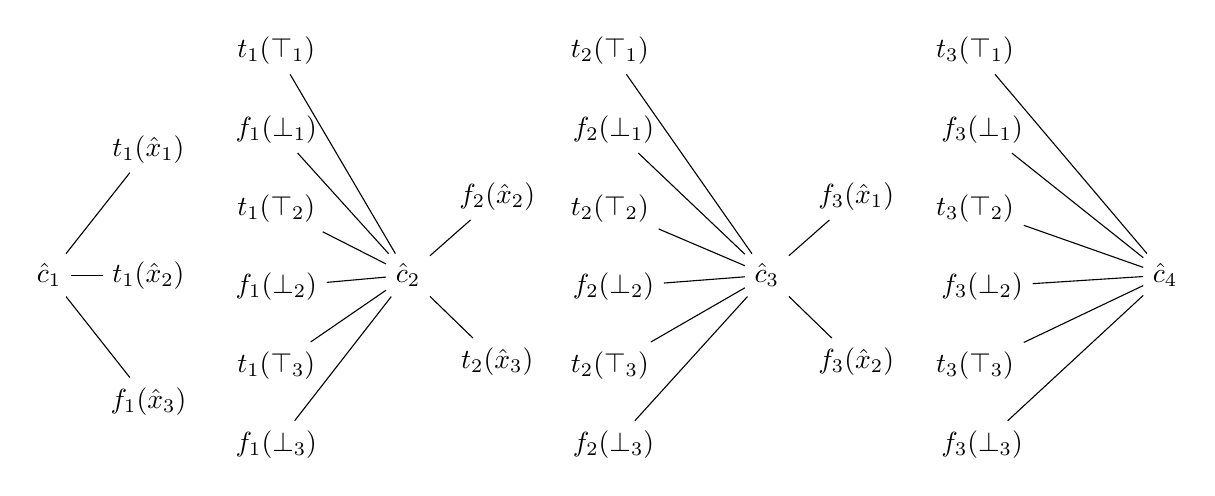
\begin{tikzpicture}[node distance=.3cm]

\node(c1){$\hat{c}_1$};

\node[right =.4cm of c1] (t1x2) {$t_1(\hat{x}_2)$};
\node[above =1cm of t1x2] (t1x1) {$t_1(\hat{x}_1)$};
\node[below =1cm of t1x2] (f1x3) {$f_1(\hat{x}_3)$};

\draw [-] (c1) to (t1x2);
\draw [-] (c1) to (t1x1);
\draw [-] (c1) to (f1x3);


\node[right =.4cm of t1x1, yshift = 0.25cm] (f11) {$f_1(\bot_1)$};
\node[above =.4cm of f11] (t11) {$t_1(\top_1)$};
\node[below =.4cm of f11] (t12) {$t_1(\top_2)$};
\node[below =.4cm of t12] (f12) {$f_1(\bot_2)$};
\node[below =.4cm of f12] (t13) {$t_1(\top_3)$};
\node[below =.4cm of t13] (f13) {$f_1(\bot_3)$};

\node[right = 4cm of c1](c2){$\hat{c}_2$};

\draw [-] (c2) to (t11);
\draw [-] (c2) to (t12);
\draw [-] (c2) to (t13);
\draw [-] (c2) to (f11);
\draw [-] (c2) to (f12);
\draw [-] (c2) to (f13);

\node[right =.25cm of c2, yshift=1cm]  (f2x2) {$f_2(\hat{x}_2)$};
\node[below =1.5cm of f2x2] (t2x3) {$t_2(\hat{x}_3)$};

\draw [-] (c2) to (f2x2);
\draw [-] (c2) to (t2x3);

\node[right =3cm of f11] (f21) {$f_2(\bot_1)$};
\node[right =3cm of t11] (t21) {$t_2(\top_1)$};
\node[right =3cm of t12] (t22) {$t_2(\top_2)$};
\node[right =3cm of f12] (f22) {$f_2(\bot_2)$};
\node[right =3cm of t13] (t23) {$t_2(\top_3)$};
\node[right =3cm of f13] (f23) {$f_2(\bot_3)$};

\node[right = 4cm of c2](c3){$\hat{c}_3$};

\draw [-] (c3) to (t21);
\draw [-] (c3) to (t22);
\draw [-] (c3) to (t23);
\draw [-] (c3) to (f21);
\draw [-] (c3) to (f22);
\draw [-] (c3) to (f23);

\node[right =.25cm of c3, yshift=1cm] (f3x1) {$f_3(\hat{x}_1)$};
\node[below =1.5cm of f3x1] (f3x2) {$f_3(\hat{x}_2)$};

\draw [-] (c3) to (f3x1);
\draw [-] (c3) to (f3x2);

\node[right =3.4cm of f21] (f31) {$f_3(\bot_1)$};
\node[right =3.4cm of t21] (t31) {$t_3(\top_1)$};
\node[right =3.4cm of t22] (t32) {$t_3(\top_2)$};
\node[right =3.4cm of f22] (f32) {$f_3(\bot_2)$};
\node[right =3.4cm of t23] (t33) {$t_3(\top_3)$};
\node[right =3.4cm of f23] (f33) {$f_3(\bot_3)$};

\node[right = 4.5cm of c3](c4){$\hat{c}_4$};

\draw [-] (c4) to (t31);
\draw [-] (c4) to (t32);
\draw [-] (c4) to (t33);
\draw [-] (c4) to (f31);
\draw [-] (c4) to (f32);
\draw [-] (c4) to (f33);

\end{tikzpicture}


\uncover<8>{

\centering
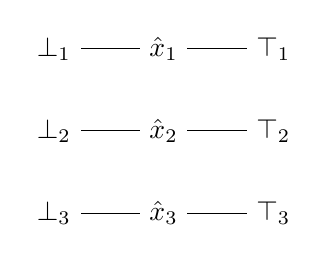
\begin{tikzpicture}[node distance=.75cm]

\node (x1) {$\hat{x}_1$};
\node [below =.5cm of x1] (x2) {$\hat{x}_2$};
\node [below =.5cm of x2] (x3) {$\hat{x}_3$};

\node [right = of x1] (t1) {$\top_1$};
\node [left = of x1] (f1) {$\bot_1$};

\draw [-] (x1) to (t1);
\draw [-] (x1) to (f1);

\node [right = of x2] (t2) {$\top_2$};
\node [left = of x2] (f2) {$\bot_2$};

\draw [-] (x2) to (t2);
\draw [-] (x2) to (f2);

\node [right = of x3] (t3) {$\top_3$};
\node [left = of x3] (f3) {$\bot_3$};

\draw [-] (x3) to (t3);
\draw [-] (x3) to (f3);

\end{tikzpicture}



}
\end{block}
}

\only<9>{
\begin{block}{Small subset corresponding to satisfying assignment}

\centering
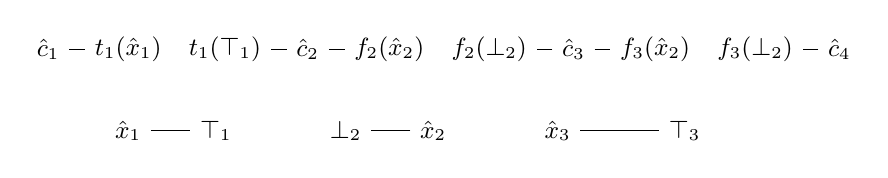
\begin{tikzpicture}
\tikzstyle{every node}=[font=\small]
\node(c1){$\hat{c}_1$};

\node[right =.2cm of c1] (t1x1) {$t_1(\hat{x}_1)$};

\draw [-] (c1) to (t1x1);

\node[right =.1cm of t1x1] (t11) {$t_1(\top_1)$};

%\draw [dashed] (t1x1) to (t11);

\node[right =.2cm of t11](c2){$\hat{c}_2$};

\draw [-] (c2) to (t11);

\node[right =.2cm of c2]  (f2x2) {$f_2(\hat{x}_2)$};

\draw [-] (c2) to (f2x2);

\node[right =.1cm of f2x2] (f22) {$f_2(\bot_2)$};

%\draw [dashed] (f2x2) to (f22);

\node[right = .2cm of f22](c3){$\hat{c}_3$};

\draw [-] (c3) to (f22);

\node[right =.2cm of c3] (f3x2) {$f_3(\hat{x}_2)$};

\draw [-] (c3) to (f3x2);

\node[right =.1cm of f3x2] (f32) {$f_3(\bot_2)$};

%\draw [dashed] (f3x2) to (f32);

\node[right =.2cm of f32](c4){$\hat{c}_4$};

\draw [-] (c4) to (f32);

\node [below =.5cm of t1x1] (x1) {$\hat{x}_1$};

\node [right =.5cm of x1] (t1) {$\top_1$};

\node [right =1cm of t1] (f2) {$\bot_2$};


\node [right =.5cm of f2] (x2) {$\hat{x}_2$};

\node [right =1cm of x2] (x3) {$\hat{x}_3$};


\node [right =1cm of x3] (t3) {$\top_3$};

\draw [-] (x1) to (t1);

\draw [-] (x2) to (f2);


\draw [-] (x3) to (t3);

\end{tikzpicture}


\end{block}
}
\end{frame}

%\section[outline]{Outline}
%\frame{\tableofcontents}

\frame{
  \frametitle{Motivation}
  \begin{block}{The Complang Style}
    \begin{columns}
      \begin{column}{7cm}
        \begin{itemize}
        \item Nicer colors
        \item Fewer boxes
        \item More room for your content!
        \end{itemize}
      \end{column}
      \begin{column}{4cm}
        
\includegraphics[width=3cm]{logo-complang}
      \end{column}
    \end{columns}
  \end{block}
  An overall great style for your presentation!
}
%-----------------------------------------------------------------------

\begin{frame}[fragile]
  \frametitle{A Listing}
  \begin{example}
    {
      % Font size for listings
      \definecolor{specparam}{rgb}{.5,0,.5}
      \definecolor{classcol}{rgb}{.1,.1,.4}
      % The table gets distractingly colourful!?
      \definecolor{methodcol}{rgb}{.1,.4,.1}
      \definecolor{commentcol}{rgb}{0,.7,0}
      \definecolor{gray}{rgb}{.2,.2,.2}

      \lstset{language=C++,
        basicstyle=\small\ttfamily,
        keywordstyle=\color{classcol},
        commentstyle=\color{commentcol},
        commentstyle=\color{gray}, 
        stringstyle=\ttfamily\color{classcol},
        emph={[2]bubble_sort,[1]return},
        emphstyle={[2]\color{methodcol}},
        emphstyle={[1]\color{classcol}} % functions/methods to be colorized
      }

\begin{lstlisting}
void bubble_sort(int* a, int n) {
  int i,j;
  for (i = 0; i < n; i++) {
    for (j = 0; j < i; j++) {
      if (a[i] > a[j]) SWAP(a[i],a[j]);
    }
  }
}
\end{lstlisting}
    }
  \end{example}
\end{frame}

%-----------------------------------------------------------------------

\frame{
  \frametitle{Thank You}
  Thank you for using the complang style!
  \vspace{3cm}

  Bug reports \& feature requests:\\
  {\tt adrian@complang.tuwien.ac.at}
}
%-----------------------------------------------------------------------

\end{document}
